\documentclass[]{article}
\usepackage{amsmath,amsfonts,amssymb,amsthm}
\usepackage{hyperref}
\usepackage[all]{xy}
\usepackage{fullpage}
\usepackage{hyperref}
\usepackage{color}
\usepackage{graphicx}
\newcommand{\taylor}[1]{{\color{blue} \sf $\spadesuit\spadesuit\spadesuit$ Taylor: [#1]}}
%\newcommand{\collab}[1]{{\color{red} \sf $\spadesuit\spadesuit\spadesuit$ collab1: [#1]}}  %Dear Collaborator, make a macro for yourself here. 
\newcommand{\todo}[1]{{\color{purple} \sf $\spadesuit\spadesuit\spadesuit$ TODO: [#1]}}

\numberwithin{equation}{section}
\newtheorem{theorem}{Theorem}[subsection]
\newtheorem{lemma}[theorem]{Lemma}
\newtheorem{corollary}[theorem]{Corollary}
\newtheorem{proposition}[theorem]{Proposition}

\theoremstyle{definition}
\newtheorem{definition}[theorem]{Definition}
\newtheorem{question}[theorem]{Question}
\newtheorem{conjecture}[theorem]{Conjecture}
\newtheorem{example}[theorem]{Example}
\newtheorem{exercise}[theorem]{Exercise}

\theoremstyle{remark}
\newtheorem{remark}[theorem]{Remark}
\newtheorem{remarks}[theorem]{Remarks}
\newtheorem{warning}[theorem]{Warning}


%opening



\begin{document}
	
\begin{center}
	{\Large \sc Dupuy -- Math 1077  --Reflections }\\
	last updated: \today
\end{center}

\noindent This document contains all of the reflection questions for Math 1077. 
There are no right or wrong answers to these questions. They are intended to get you thinking about a certain topic before we engage with them in class.
\vspace{1em}

\noindent {\bf WARNING}: Prior to their being assigned a due date reflection questions are subject to change! This includes, but is not limited, to the order in which reflection questions are given and title of the reflections. Some of the reflections might not be assigned at all!

\subsection{Calculators and Really Small Numbers }
We often take calculators for granted. 
Find you nearest calculator (google, iPhone, or laptop will work) and input $31+10^{-16}$, that is, try to get it to perform the addition $31 + 0.0000000000000001$.
Explain what computer you used and what happened? 
Try it on another system. 
Why do you think this happens?
What is the largest number such that 1 plus that number returns 1 on that device? [there are some devices where this won't work, I know this works on google.]

\subsection{Expected Values Are Everywhere }
Expected values are everywhere.
They can be used in games, psychology experiments, interpersonal relationships, business, biology, and elsewhere. 
Give an example of an expected value that you care about? This can be from a game you play or from something you like to collect or anything really. 

\subsection{Bernoulli's Game}\footnote{Ellenberg ``St Petersburg and Ellsburg'' pg 242}
Consider the following five dollar carnival game. 
In this game, you are asked to repeatedly toss a coin and the game stops the first time you flip heads. 
The payout structure is as follows:
\begin{itemize}
	\item if you flip heads (H) your first try you get \$1. 
	\item if you flip tails then heads (TH) you get \$2.
	\item if you flip two tails then a heads (TTH) you get \$4. 
	\item if you flip TTTH you get \$8.
	\item $\cdots$
\end{itemize}	
The pattern keeps going with the payout doubling for each tail you flip in a row. 
Should you play this game?
How much should you pay to play this game?

\subsection{Flipping Coins }
Produce a sheet of paper with 200 coin flips recording a sequential number of heads and tails. There are two ways you can do this. 
You can cheat and just write down a bunch of heads and tails or you actually flip a coin 200 times. 
All I ask is that you don't mix these two ways of completing this assignment.
Either completely cheat and just write down random heads and tails or you actually flip coins and do this for the entire 200 flips.
When you submit the assignment don't say which method you used.

\subsection{The Monty Hall Problem } 
\begin{enumerate}
	\item Suppose you are going to buy a lottery tickey and the only prize is the jackpot. In the game you select six numbers 1-50. Which ticket is better the ticket with 1,1,1,1,1,1 or the ticket with 12,26,3,50,24,27? Why or why not?
	\item Suppose you are flipping a coin and you flip 10 heads in a row. Is it more likely that you flip a tails the next time?
	\item You flip 5 coins. Which outcome is more likely HHHHH or HTHTH?
	\item You are the contestant an \emph{Let's Make A Deal} with host Monty Hall. In this game there are three doors. Behind two of the doors there are goats and behind one of the doors is a brand new car. Your job is to guess which door has the car and if you get it right, you get the car. Monty asks you to select a door. After your selection he reveals goats behind one of the doors. You are allowed to stay with your current door or switch. What should you do? Should you stay with your current door? Should you switch to the new door? Does it matter?
\end{enumerate}

\subsection{What is Ranked Choice Voting? }
In 2009 Burlington had an election for Mayor in which there were three candidates. At the time the city implemented "ranked choice voting" which is a system in which voters submit a ballot which ranks their perferred order of candidates. How do you suppose this worked? Make up some rules that would allow you to elect a mayor to take into account the voters will using these ranked ballots. How would you determine the winner if you were allowed to make up a voting system? Why?
	
\subsection{Seven Bridges of Koenigsburg }
Euler lived in the city of \href{https://goo.gl/maps/h28p2rEpXZGGkn9M6}{Koenigsberg} (modern day Kaliningrad). The city had a system of bridges as mapped out below in Figure\ref{F:seven-bridges}. 
Euler wanted to find a route through the city to walk across each one of the bridges exactly once in the city. 
How can Euler achieve such a route? Make a map and try making a route that achieves this. 

\begin{figure}[h]
	\begin{center}
		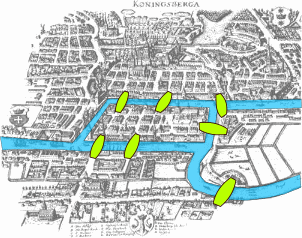
\includegraphics[scale=0.5]{konigsberg_bridges.png}
	\end{center}
\caption{The city of Koenigsburg and its seven bridges.}\label{F:seven-bridges}
\end{figure}
	
\subsection{3 Houses and 3 Utlilities }
	My 5th grade teacher math Mrs. Kelly gave me the following problem in 1995: 
	There are three houses and three utilities as pictured below.
	Draw a line connecting each of the three houses to each of the three utilities without any of the lines cross each other. Explain what is going on in this problem.
	\begin{figure}[h]
		\begin{center}
			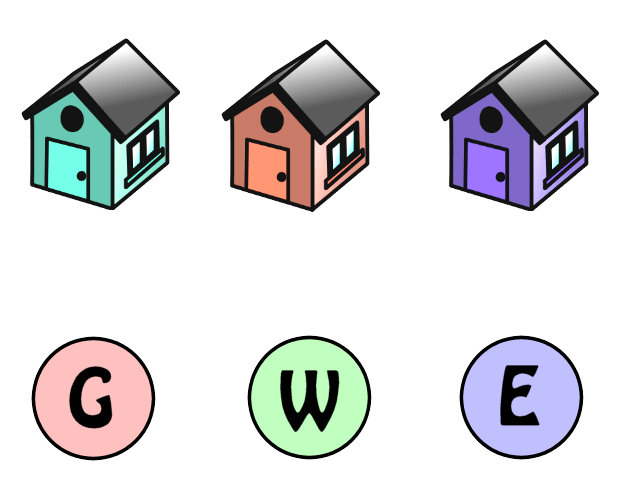
\includegraphics[scale=0.25]{three-houses.png}
		\end{center}
		\caption{A image of the three houses and three utilities problem.  Image taken from \href{http://puzzles.nigelcoldwell.co.uk/twentysix.htm}{Nigel Coldwell's webpage.} }
	\end{figure}
	
\subsection{Prisoner Problem }
There are 50 prisoners numbered 1 through 50.
There are 50 boxes numbered 1 through 50 in a room. 
Each of the numbers 1-50 are placed in the boxes at random with each number appearing in a box exactly once (so for example the number 7 could be placed in box 20).
The Warden then plays a game for the prisoners freedom: each prisoner is led into the room one at a time and is asked to find their own number.
They get to open 25 boxes.
After a prisoner leaves the room, the boxes and numbers are reset to their original configuration (so all of the prisoners get the same setup). 
If \emph{all} of the prisoners find their number they will all be set free.

The prisoners are allowed to communicate beforehand to come up with a strategy but are not allowed to communicate after the game has started. What strategy should they use? (Spoiler: there exists a strategy that works about 30\% of the time)


\iffalse 
\subsection{}	
	\taylor{TBD $p$-value}
	
\subsection{}
	
	\taylor{TBD regression to the mean}
	
\subsection{M\"obius Band}
What do you think will happen if we take a M\"obius band and cut it down the middle?

\fi 
%\bibliographystyle{amsalpha}
%\bibliography{mydocument.bib}

\end{document}
